\documentclass[tikz,border=15pt]{standalone}
\usepackage{tikz}
\usepackage{amsmath}
\usepackage{amssymb}
\usetikzlibrary{shapes.geometric, arrows.meta, positioning, calc, backgrounds, fit, shadows.blur}

\definecolor{navyDark}{HTML}{0B2545}
\definecolor{navyLight}{HTML}{F0F4F8}
\definecolor{navyBorder}{HTML}{134074}

\definecolor{crimsonDark}{HTML}{78281F}
\definecolor{crimsonLight}{HTML}{FDF2E9}
\definecolor{crimsonBorder}{HTML}{C0392B}

\definecolor{emeraldDark}{HTML}{0E6251}
\definecolor{emeraldLight}{HTML}{E8F8F5}
\definecolor{emeraldBorder}{HTML}{16A085}

\definecolor{slateDark}{HTML}{2C3E50}
\definecolor{slateLight}{HTML}{F8F9FA}
\definecolor{slateBorder}{HTML}{BDC3C7}

\begin{document}
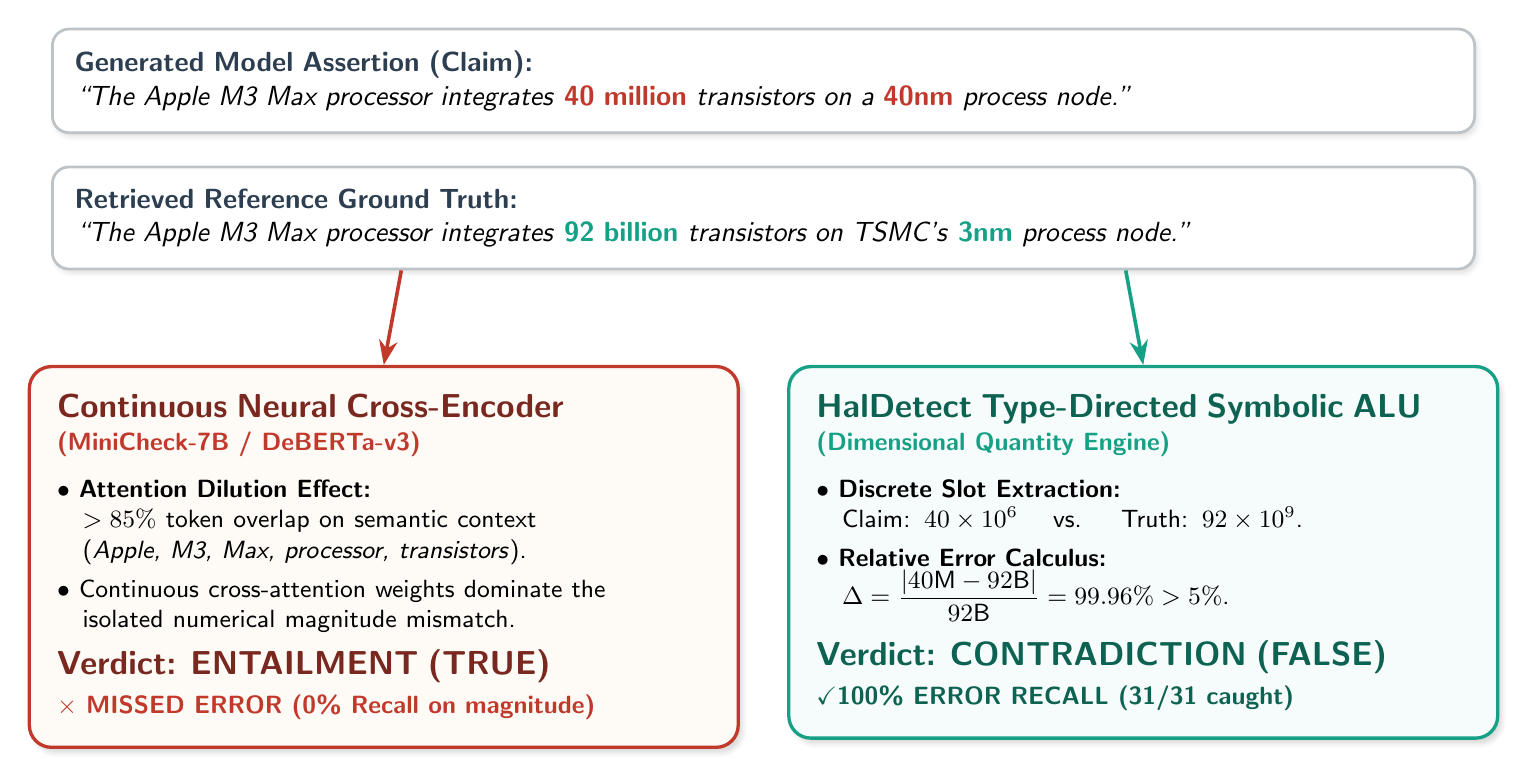
\begin{tikzpicture}[
    font=\sffamily,
    >=Stealth,
    claimbox/.style={
        draw=slateBorder, fill=white, line width=1.0pt, rounded corners=6pt,
        blur shadow={shadow blur steps=4, shadow xshift=1pt, shadow yshift=-1.5pt, shadow opacity=12},
        align=left, inner sep=8pt
    },
    branchcard/.style={
        draw=#1Border, fill=#1Light!40, line width=1.2pt, rounded corners=8pt,
        blur shadow={shadow blur steps=5, shadow xshift=1.5pt, shadow yshift=-2pt, shadow opacity=15},
        align=left, inner sep=10pt
    },
    wire/.style={
        ->, line width=1.3pt, draw=#1Border
    }
]

% Claim & Ground Truth Boxes
\node[claimbox, text width=17.5cm] (claim) at (9.0, 4.6) {
    \textbf{\color{slateDark} Generated Model Assertion (Claim):}\\
    \textit{``The Apple M3 Max processor integrates \textbf{\color{crimsonBorder}40 million} transistors on a \textbf{\color{crimsonBorder}40nm} process node.''}
};

\node[claimbox, text width=17.5cm, below=0.4cm of claim] (ground) {
    \textbf{\color{slateDark} Retrieved Reference Ground Truth:}\\
    \textit{``The Apple M3 Max processor integrates \textbf{\color{emeraldBorder}92 billion} transistors on TSMC's \textbf{\color{emeraldBorder}3nm} process node.''}
};

% Left: Neural Cross-Encoder Failure Branch
\node[branchcard=crimson, text width=8.3cm, below left=1.2cm and 0.3cm of ground.south, anchor=north east] (left_box) {
    \textbf{\color{crimsonDark}\large Continuous Neural Cross-Encoder}\\
    \textbf{\color{crimsonBorder}\small (MiniCheck-7B / DeBERTa-v3)}\\
    \vspace{6pt}
    \small $\bullet$ \textbf{Attention Dilution Effect:}\\
    \quad $>85\%$ token overlap on semantic context\\
    \quad (\textit{Apple, M3, Max, processor, transistors}).\\
    \vspace{3pt}
    \small $\bullet$ Continuous cross-attention weights dominate the\\
    \quad isolated numerical magnitude mismatch.\\
    \vspace{6pt}
    \textbf{\color{crimsonDark}\large Verdict: ENTAILMENT (TRUE)}\\
    \vspace{2pt}
    \textbf{\color{crimsonBorder}\small $\times$ MISSED ERROR (0\% Recall on magnitude)}
};

% Right: Symbolic SI ALU Success Branch
\node[branchcard=emerald, text width=8.3cm, below right=1.2cm and 0.3cm of ground.south, anchor=north west] (right_box) {
    \textbf{\color{emeraldDark}\large HalDetect Type-Directed Symbolic ALU}\\
    \textbf{\color{emeraldBorder}\small (Dimensional Quantity Engine)}\\
    \vspace{6pt}
    \small $\bullet$ \textbf{Discrete Slot Extraction:}\\
    \quad Claim: $40\times 10^6$ \quad vs. \quad Truth: $92\times 10^9$.\\
    \vspace{3pt}
    \small $\bullet$ \textbf{Relative Error Calculus:}\\
    \quad $\Delta = \dfrac{|40\text{M} - 92\text{B}|}{92\text{B}} = 99.96\% > 5\%$.\\
    \vspace{6pt}
    \textbf{\color{emeraldDark}\large Verdict: CONTRADICTION (FALSE)}\\
    \vspace{2pt}
    \textbf{\color{emeraldDark}\small \checkmark 100\% ERROR RECALL (31/31 caught)}
};

\draw[wire=crimson] ($(ground.south) - (4.6, 0)$) -- (left_box.north);
\draw[wire=emerald] ($(ground.south) + (4.6, 0)$) -- (right_box.north);

\end{tikzpicture}
\end{document}
